
%%%%%%%%%%%%%%%%%%%%%%% 附录 %%%%%%%%%%%%%%%%%%%%%%%%%

% 添加附录, 如不需要可以把附录部分注释
\appendix

%\fangsong %设置字体为仿宋

% 附录正文
\section{这是第一个附录}

\subsection{附录A的小节}

这里是附录环境.

附录公式及编号
\begin{equation}\label{eq:abc}
  a^2+b^2=c^2.
\end{equation}

附录的插图: 如图~\ref{fig:sinx2}.
\begin{figure}[htp!]
  \centering
  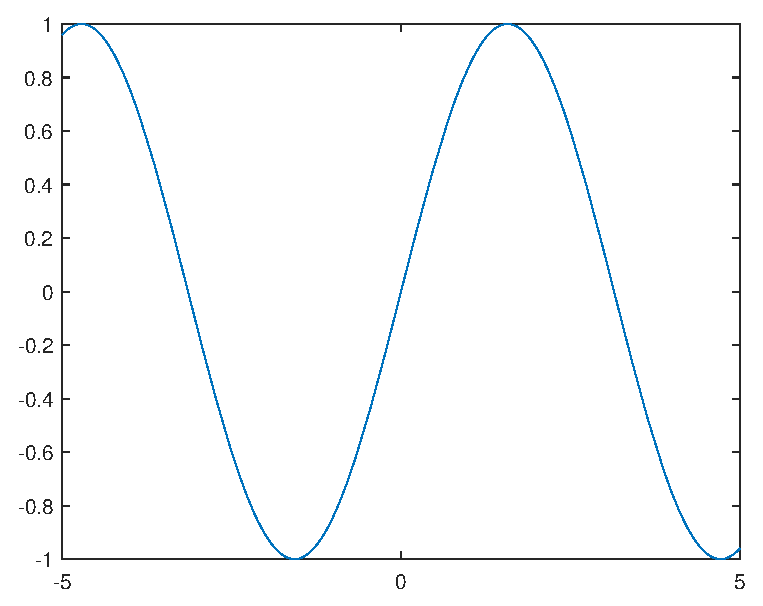
\includegraphics[width=0.45\linewidth]{image1.eps}
  \caption{函数 $y=\sin(x)$ 的图像}\label{fig:sinx2}
\end{figure}

附录的表格: 表~\ref{tab:heightweight2}. 通过 \verb|autoref| 引用表格: \autoref{tab:heightweight2}.

\begin{table}[!htp]
\centering
% PLCR已经定义
\caption{某校学生升高体重样本}
\label{tab:heightweight2}
\begin{tabularx}{0.9\textwidth}{lCCC}
   \toprule
	序号 & 年龄 & 身高 & 体重 \\
	\midrule
	001 & 15 & 156 & 42 \\
	002 & 16 & 158 & 45 \\
	003 & 14 & 162 & 48 \\
	004 & 15 & 163 & 50 \\
    \cmidrule{2-4}
	平均 & 15 & 159.75 & 46.25 \\
	\bottomrule
\end{tabularx}
\end{table}


\section{程序源代码}

\subsection{MATLAB 代码环境}

这是 MATLAB 程序代码高亮环境.

% set code font
%basicstyle=\footnotesize\fontspec{Courier New}
%basicstyle=\footnotesize\fontspec{Consolas}

\begin{lstlisting}[style=matlab,basicstyle=\footnotesize\fontspec{Courier New},title={MATLAB code}]
% Euler method for the ODE model
% u'(x)=x^2+x-u, x in [0,1]
% Initial condition: u(0)=0 ;
% Exact solution: u(x)=-exp(-x)+x^2-x+1.
clear all;  clf
h=0.1;
x=0:h:1;
N=length(x)-1;
u(1)=0;                        % initial value
fun=@(t,u) t.^2+t-u;           % RHS

for n=1:N
    u(n+1)=u(n)+h.*fun(x(n),u(n));
end

ue=-exp(-x)+x.^2-x+1;          % exact solution
plot(x,ue,'b-',x,u,'r+','LineWidth',1)
legend('Exact','Numerical','location','North')
%title('Euler method','fontsize',12)
set(gca,'fontsize',12)
xlabel('x','fontsize',16), ylabel('u','fontsize',16,'Rotation',0)
\end{lstlisting}

\subsection{Python 代码环境}

这是 Python 程序代码高亮环境.

\begin{lstlisting}[style=python,basicstyle=\footnotesize\fontspec{Consolas},title={Python code}]
#PythonDraw.py
import turtle as t
t.setup(650, 350, 200, 200)
t.penup()
t.fd(-250)
t.pendown()
t.pensize(25)
t.pencolor("purple color")
t.seth(-40)
for i in range(4):
    t.circle(40, 80)
    t.circle(-40, 80)
t.circle(40, 80/2)
t.fd(40)
t.circle(16, 180)
t.fd(40 * 2/3)
t.done()
\end{lstlisting}


